\clearpage
\setcounter{page}{1}
\setcounter{section}{0}  % Reset section numbering
\setcounter{figure}{0}   % Reset figure numbering
\setcounter{table}{0}    % Reset table numbering
\setcounter{equation}{0} % Reset equation numbering
\maketitlesupplementary




\section{Triage agent}

Figure \ref{fig:triage} illustrates the architecture of the Triage Agent. To evaluate its effectiveness, we compared the performance of the Triage Agent against three MIL-based benchmark methods \cite{ilse2018attentionbaseddeepmultipleinstance, li2021dualstreammultipleinstancelearning, shao2021transmil} for detecting Class 1 vs. Non-Class 1 cases in the M-Path dataset (details in Section \ref{data-mpath}). As summarized in Table \ref{tab:triageexperiments}, PathFinder's Triage Agent, designed to assess whether a WSI is risky, outperforms the baseline methods.

\begin{figure*}[ht]
\begin{center}
\includegraphics[width=\linewidth]{figures/Triage-agent.png}
\end{center}
   \caption{Overview of the Triage Agent architecture. Definitions of $M$ and $H$ can be found in Section \ref{sec:methods}.}
\label{fig:triage}
\end{figure*}


\begin{table}[ht]
  \centering
  \scriptsize
  \begin{tabular}{lccc}
    \toprule
    Method & Class 1 F1 & Non-Class 1 F1 & Overall Accuracy \\
    \midrule
    AMIL \cite{ilse2018attentionbaseddeepmultipleinstance} & 0.16 & 0.83 & 0.71 \\
    DSMIL \cite{li2021dualstreammultipleinstancelearning} & 0.35 & 0.86 & 0.77 \\
    TransMIL \cite{shao2021transmil} & 0.40 & 0.90 & 0.83 \\
    \midrule
    \textbf{Triage Agent} & \textbf{0.57} & \textbf{0.95} & \textbf{0.91} \\
    \bottomrule
  \end{tabular}
  \caption{Comparison of Triage Agent with benchmark methods on Class 1 vs. Non-Class 1 classification}
  \label{tab:triageexperiments}
\end{table}

\section{VLM-based Navigation Agent}
\label{supp:llava-nav}

Our initial approach to designing the Navigator Agent explored a multi-modal architecture based on the LLaVA framework \cite{liu2023improved}. This design aimed to enable direct reasoning over image latents through an LLM. The architecture consisted of two main components:

\begin{enumerate}
    \item A U-Net encoder \cite{ronneberger2015u} pre-trained on pathologist viewing behavior data (M-Path, details in Section \ref{data-mpath}), which served as the image encoder
    \item The LLaMA-7B language model \cite{touvron2023llama}, which acted as the reasoning component
\end{enumerate}

\subsection{Training Process and Architecture}
We first trained a complete U-Net on the M-Path dataset to learn meaningful representations of WSIs. For the Navigator implementation, we removed the U-Net's decoder and retained only the encoder portion. This encoder was then integrated with LLaMA-7B following the LLaVA framework. The combined model was trained using instruction tuning, where each training instance consisted of:
\begin{itemize}
    \item Input: A WSI and a list of previous observations and their descriptions obtained from the Description agent
    \item Output: Grid coordinates (row and column) identifying regions of interest within the WSI
\end{itemize}

The underlying hypothesis was that the LLM could effectively process the U-Net-encoded latent representations to identify diagnostically relevant grid coordinates directly.

\subsection{Limitations and Challenges with a LLaVA-based Navigator}
This approach encountered several significant limitations:

\begin{enumerate}
    \item \textbf{Data Scarcity}: The available navigation training dataset proved insufficient for the model to learn robust region selection strategies.
    
    \item \textbf{Overfitting Patterns}: The model exhibited clear signs of overfitting:
    \begin{itemize}
        \item Consistently selecting patches from the central regions of WSIs, regardless of input
        \item Generating repetitive patch selections
        \item Failing to generalize to novel slide patterns
    \end{itemize}
\end{enumerate}

\subsection{Architectural Pivot}
These limitations led us to revise our approach fundamentally. Instead of requiring the LLM to reason directly from latent representations, we returned to utilizing the complete U-Net architecture (including the decoder), and leverage the decoded attention maps for direct region sampling. This proved to be more robust with limited training data, and we simply conditioned our U-Net with the descriptions from the Description Agent to have the feedback loop between the agents. This experience highlighted the challenges of applying LLMs to specialized medical tasks with constrained training data, even when pre-training sub-modules (like our U-Net encoder in this case).



\section{Description agent}

We generated fine-tuning data for the Description Agent by prompting GPT-4 to extract short and concise histopathology findings from provided text. Figure \ref{fig:descriptionprompt} illustrates the prompt used and a sample of the data generated for fine-tuning the Description Agent.

\begin{figure*}[h]
\begin{center}
\includegraphics[width=0.9\linewidth]{figures/description-prompt.png}
\end{center}
   \caption{GPT-4 prompt to generate instruction-tuning dataset for the Description Agent.}
\label{fig:descriptionprompt}
\end{figure*}






\section{Evaluation and experiments}

This section provides details on the qualitative analysis conducted by pathologists and the prompt for our LLM-prompting experiments.

\subsection{Qualitative Analysis of Descriptions Assessed by Pathologists}
\label{supp:pathologists-analysis}

To evaluate the quality of the descriptions generated by the Description Agent, we cropped the region of interest from 25 WSIs from M-Path dataset and generated descriptions for these regions using three models: PathFinder's Description Agent, GPT-4o, and LLaVa-Med. Since our Description Agent is fine-tuned to produce short and concise descriptions, we ensured a fair comparison by prompting LLaVa-Med and GPT-4o with the instruction: \textit{Describe the histology image concisely in less than 20 words}. We conducted a survey involving two pathologists who were asked to answer the following two questions regarding descriptions produced by the three models. The study was conducted in a double-blind, randomized manner to ensure unbiased results:

\begin{enumerate}
    \item \textbf{Selection}: Please select the description that you believe best matches the content of the image. (Options: Model A, Model B, Model C)
    \item \textbf{Reason for Preference}: Please choose the primary reason for your preference. You may select more than one option if applicable. If Other, please specify.
    \begin{itemize}
        \item \textbf{Correctness}: The description accurately reflects the features of the image.
        \item \textbf{Detail}: The description provides a comprehensive analysis of the image.
        \item \textbf{Relevance}: The description emphasizes the most pertinent aspects of the image.
        \item \textbf{Other}: Please specify.
    \end{itemize}
\end{enumerate}

\begin{figure*}[h]
    \centering
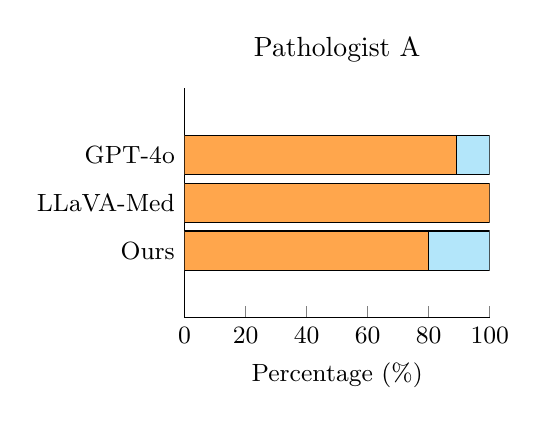
\begin{tikzpicture}
    \begin{axis}[
        width=0.45\linewidth,
        height=4.5cm,
        xbar stacked,
        bar width=0.5cm,
        xmin=0, xmax=100,
        axis x line*=bottom,
        axis y line*=left,
        ymin=-0.5, ymax=2.5,
        ytick=data,
        yticklabels={Ours, LLaVA-Med, GPT-4o},
        enlarge y limits=0.3,
        xlabel={Percentage (\%)},
        title={Pathologist A},
        tick label style={font=\small},
        label style={font=\small},
    ]
    % Pathologist A ratings
    \addplot[fill=orange!70] coordinates {(80,0) (100,1) (89,2)}; % Reason 1
    \addplot[fill=blue!40] coordinates {(0,0) (0,1) (0,2)}; % Reason 2
    \addplot[fill=cyan!30] coordinates {(20,0) (0,1) (11,2)}; % Reason 3
    
    % \legend{Reason 1, Reason 2, Reason 3}
    \end{axis}
\end{tikzpicture}
\hfill
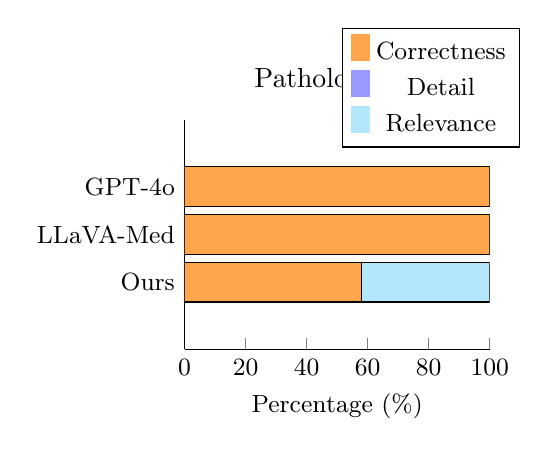
\begin{tikzpicture}
    \begin{axis}[
        width=0.45\linewidth,
        height=4.5cm,
        xbar stacked,
        bar width=0.5cm,
        xmin=0, xmax=100,
        axis x line*=bottom,
        axis y line*=left,
        ymin=-0.5, ymax=2.5,
        ytick=data,
        yticklabels={Ours, LLaVA-Med, GPT-4o},
        enlarge y limits=0.3,
        xlabel={Percentage (\%)},
        title={Pathologist B},
        tick label style={font=\small},
        label style={font=\small},
        legend style={font=\small, at={(1.1,1.4)}, anchor=north east, legend columns=1},
        legend image code/.code={
            \draw[#1, draw=none] (0cm,-0.1cm) rectangle (0.25cm,0.25cm);
        },
    ]
    % Pathologist B ratings
    \addplot[fill=orange!70] coordinates {(58,0) (100,1) (100,2)}; % Reason 1
    \addplot[fill=blue!40] coordinates {(0,0) (50,1) (40,2)}; % Reason 2
    \addplot[fill=cyan!30] coordinates {(42,0) (20,1) (30,2)}; % Reason 3
    
    \legend{Correctness, Detail, Relevance}
    \end{axis}
\end{tikzpicture}

\caption{Expert human pathologist preferences for each model, segmented by the reasons for their choices. Each subplot corresponds to one pathologist and shows their ratings for PathFinder (Ours), LLaVA-Med, and GPT-4o.}
\label{fig:pathologist-analysis-reason}
\end{figure*}


Figure \ref{fig:pathologist-analysis-reason} illustrates the distribution of reasons selected by pathologists for preferring each model. As shown, none of the models were preferred for their level of detail, which aligns with expectations since the models were specifically prompted to generate short and concise descriptions, inherently limiting detailed information. The majority of preferences were based on the correctness of the descriptions.



\subsection{Prompt used for pre-trained LLM experiments}
\label{supp:diagnosis-llm-prompting}
The following prompt was used in our experiments with pre-trained LLMs serving as the Diagnosis Agent to make a diagnosis based on the provided \textit{descriptions}:

\noindent\textbf{Prompt:} Answer the following question related to skin cancer. Only use one of the four options given at the end. \newline
The image descriptions below are extracted from different patches from the same whole slide image (WSI), please tell me which class the image belongs to:\newline
\textit{\{descriptions\}}\newline
The options are: \\
"diagnosis: (I) mildly dysplastic nevi, moderately dysplastic nevi"\\
"diagnosis: (II) melanoma in situ and severely dysplastic nevi"\\
"diagnosis: (III) invasive melanoma stage pT1a"\\
"diagnosis: (IV) advanced invasive melanoma stage $\geq$ pT1b"\\
Only output the complete text of the option you choose. Don't add any more words.
